% Options for packages loaded elsewhere
\PassOptionsToPackage{unicode}{hyperref}
\PassOptionsToPackage{hyphens}{url}
\PassOptionsToPackage{dvipsnames,svgnames,x11names}{xcolor}
%
\documentclass[
  letterpaper,
  DIV=11,
  numbers=noendperiod]{scrreprt}

\usepackage{amsmath,amssymb}
\usepackage{lmodern}
\usepackage{iftex}
\ifPDFTeX
  \usepackage[T1]{fontenc}
  \usepackage[utf8]{inputenc}
  \usepackage{textcomp} % provide euro and other symbols
\else % if luatex or xetex
  \usepackage{unicode-math}
  \defaultfontfeatures{Scale=MatchLowercase}
  \defaultfontfeatures[\rmfamily]{Ligatures=TeX,Scale=1}
\fi
% Use upquote if available, for straight quotes in verbatim environments
\IfFileExists{upquote.sty}{\usepackage{upquote}}{}
\IfFileExists{microtype.sty}{% use microtype if available
  \usepackage[]{microtype}
  \UseMicrotypeSet[protrusion]{basicmath} % disable protrusion for tt fonts
}{}
\makeatletter
\@ifundefined{KOMAClassName}{% if non-KOMA class
  \IfFileExists{parskip.sty}{%
    \usepackage{parskip}
  }{% else
    \setlength{\parindent}{0pt}
    \setlength{\parskip}{6pt plus 2pt minus 1pt}}
}{% if KOMA class
  \KOMAoptions{parskip=half}}
\makeatother
\usepackage{xcolor}
\setlength{\emergencystretch}{3em} % prevent overfull lines
\setcounter{secnumdepth}{5}
% Make \paragraph and \subparagraph free-standing
\ifx\paragraph\undefined\else
  \let\oldparagraph\paragraph
  \renewcommand{\paragraph}[1]{\oldparagraph{#1}\mbox{}}
\fi
\ifx\subparagraph\undefined\else
  \let\oldsubparagraph\subparagraph
  \renewcommand{\subparagraph}[1]{\oldsubparagraph{#1}\mbox{}}
\fi


\providecommand{\tightlist}{%
  \setlength{\itemsep}{0pt}\setlength{\parskip}{0pt}}\usepackage{longtable,booktabs,array}
\usepackage{calc} % for calculating minipage widths
% Correct order of tables after \paragraph or \subparagraph
\usepackage{etoolbox}
\makeatletter
\patchcmd\longtable{\par}{\if@noskipsec\mbox{}\fi\par}{}{}
\makeatother
% Allow footnotes in longtable head/foot
\IfFileExists{footnotehyper.sty}{\usepackage{footnotehyper}}{\usepackage{footnote}}
\makesavenoteenv{longtable}
\usepackage{graphicx}
\makeatletter
\def\maxwidth{\ifdim\Gin@nat@width>\linewidth\linewidth\else\Gin@nat@width\fi}
\def\maxheight{\ifdim\Gin@nat@height>\textheight\textheight\else\Gin@nat@height\fi}
\makeatother
% Scale images if necessary, so that they will not overflow the page
% margins by default, and it is still possible to overwrite the defaults
% using explicit options in \includegraphics[width, height, ...]{}
\setkeys{Gin}{width=\maxwidth,height=\maxheight,keepaspectratio}
% Set default figure placement to htbp
\makeatletter
\def\fps@figure{htbp}
\makeatother
\newlength{\cslhangindent}
\setlength{\cslhangindent}{1.5em}
\newlength{\csllabelwidth}
\setlength{\csllabelwidth}{3em}
\newlength{\cslentryspacingunit} % times entry-spacing
\setlength{\cslentryspacingunit}{\parskip}
\newenvironment{CSLReferences}[2] % #1 hanging-ident, #2 entry spacing
 {% don't indent paragraphs
  \setlength{\parindent}{0pt}
  % turn on hanging indent if param 1 is 1
  \ifodd #1
  \let\oldpar\par
  \def\par{\hangindent=\cslhangindent\oldpar}
  \fi
  % set entry spacing
  \setlength{\parskip}{#2\cslentryspacingunit}
 }%
 {}
\usepackage{calc}
\newcommand{\CSLBlock}[1]{#1\hfill\break}
\newcommand{\CSLLeftMargin}[1]{\parbox[t]{\csllabelwidth}{#1}}
\newcommand{\CSLRightInline}[1]{\parbox[t]{\linewidth - \csllabelwidth}{#1}\break}
\newcommand{\CSLIndent}[1]{\hspace{\cslhangindent}#1}

\KOMAoption{captions}{tableheading}
\makeatletter
\@ifpackageloaded{tcolorbox}{}{\usepackage[many]{tcolorbox}}
\@ifpackageloaded{fontawesome5}{}{\usepackage{fontawesome5}}
\definecolor{quarto-callout-color}{HTML}{909090}
\definecolor{quarto-callout-note-color}{HTML}{0758E5}
\definecolor{quarto-callout-important-color}{HTML}{CC1914}
\definecolor{quarto-callout-warning-color}{HTML}{EB9113}
\definecolor{quarto-callout-tip-color}{HTML}{00A047}
\definecolor{quarto-callout-caution-color}{HTML}{FC5300}
\definecolor{quarto-callout-color-frame}{HTML}{acacac}
\definecolor{quarto-callout-note-color-frame}{HTML}{4582ec}
\definecolor{quarto-callout-important-color-frame}{HTML}{d9534f}
\definecolor{quarto-callout-warning-color-frame}{HTML}{f0ad4e}
\definecolor{quarto-callout-tip-color-frame}{HTML}{02b875}
\definecolor{quarto-callout-caution-color-frame}{HTML}{fd7e14}
\makeatother
\makeatletter
\makeatother
\makeatletter
\@ifpackageloaded{bookmark}{}{\usepackage{bookmark}}
\makeatother
\makeatletter
\@ifpackageloaded{caption}{}{\usepackage{caption}}
\AtBeginDocument{%
\ifdefined\contentsname
  \renewcommand*\contentsname{Table of contents}
\else
  \newcommand\contentsname{Table of contents}
\fi
\ifdefined\listfigurename
  \renewcommand*\listfigurename{List of Figures}
\else
  \newcommand\listfigurename{List of Figures}
\fi
\ifdefined\listtablename
  \renewcommand*\listtablename{List of Tables}
\else
  \newcommand\listtablename{List of Tables}
\fi
\ifdefined\figurename
  \renewcommand*\figurename{Figure}
\else
  \newcommand\figurename{Figure}
\fi
\ifdefined\tablename
  \renewcommand*\tablename{Table}
\else
  \newcommand\tablename{Table}
\fi
}
\@ifpackageloaded{float}{}{\usepackage{float}}
\floatstyle{ruled}
\@ifundefined{c@chapter}{\newfloat{codelisting}{h}{lop}}{\newfloat{codelisting}{h}{lop}[chapter]}
\floatname{codelisting}{Listing}
\newcommand*\listoflistings{\listof{codelisting}{List of Listings}}
\makeatother
\makeatletter
\@ifpackageloaded{caption}{}{\usepackage{caption}}
\@ifpackageloaded{subcaption}{}{\usepackage{subcaption}}
\makeatother
\makeatletter
\@ifpackageloaded{tcolorbox}{}{\usepackage[many]{tcolorbox}}
\makeatother
\makeatletter
\@ifundefined{shadecolor}{\definecolor{shadecolor}{rgb}{.97, .97, .97}}
\makeatother
\makeatletter
\makeatother
\ifLuaTeX
  \usepackage{selnolig}  % disable illegal ligatures
\fi
\IfFileExists{bookmark.sty}{\usepackage{bookmark}}{\usepackage{hyperref}}
\IfFileExists{xurl.sty}{\usepackage{xurl}}{} % add URL line breaks if available
\urlstyle{same} % disable monospaced font for URLs
\hypersetup{
  pdftitle={巫雨洋的学习日记},
  pdfauthor={Yuyang Wu},
  colorlinks=true,
  linkcolor={blue},
  filecolor={Maroon},
  citecolor={Blue},
  urlcolor={Blue},
  pdfcreator={LaTeX via pandoc}}

\title{巫雨洋的学习日记}
\author{Yuyang Wu}
\date{2023/1/26}

\begin{document}
\maketitle
\ifdefined\Shaded\renewenvironment{Shaded}{\begin{tcolorbox}[borderline west={3pt}{0pt}{shadecolor}, interior hidden, boxrule=0pt, frame hidden, sharp corners, enhanced, breakable]}{\end{tcolorbox}}\fi

\renewcommand*\contentsname{Table of contents}
{
\hypersetup{linkcolor=}
\setcounter{tocdepth}{2}
\tableofcontents
}
\bookmarksetup{startatroot}

\hypertarget{preface}{%
\chapter*{Preface}\label{preface}}
\addcontentsline{toc}{chapter}{Preface}

This is a Learning Diary for CASA0023

\bookmarksetup{startatroot}

\hypertarget{a-brief-summary}{%
\chapter*{A Brief Summary}\label{a-brief-summary}}
\addcontentsline{toc}{chapter}{A Brief Summary}

\bookmarksetup{startatroot}

\hypertarget{week1}{%
\chapter{WEEK1}\label{week1}}

\hypertarget{key-points}{%
\section{Key Points}\label{key-points}}

\hypertarget{what-is-remote-sensing}{%
\subsection{What is Remote Sensing}\label{what-is-remote-sensing}}

\textbf{Sensors and remote sensing platforms}

Sensors are devices that collect and record information about
electromagnetic radiation capabilities and are mounted on remote sensing
platforms. Sensors are classified according to how they work and into
active and passive sensors. Remote sensing platforms are mainly divided
into, ground, air and space based remote sensing platforms.

\textbf{Electromagentic waves}

Electromagnetic waves can be classified into different bands according
to the order of their wavelength or frequency in a vacuum. The following
diagram shows the electromagnetic spectrum commonly used in remote
sensing.

\begin{figure}

{\centering 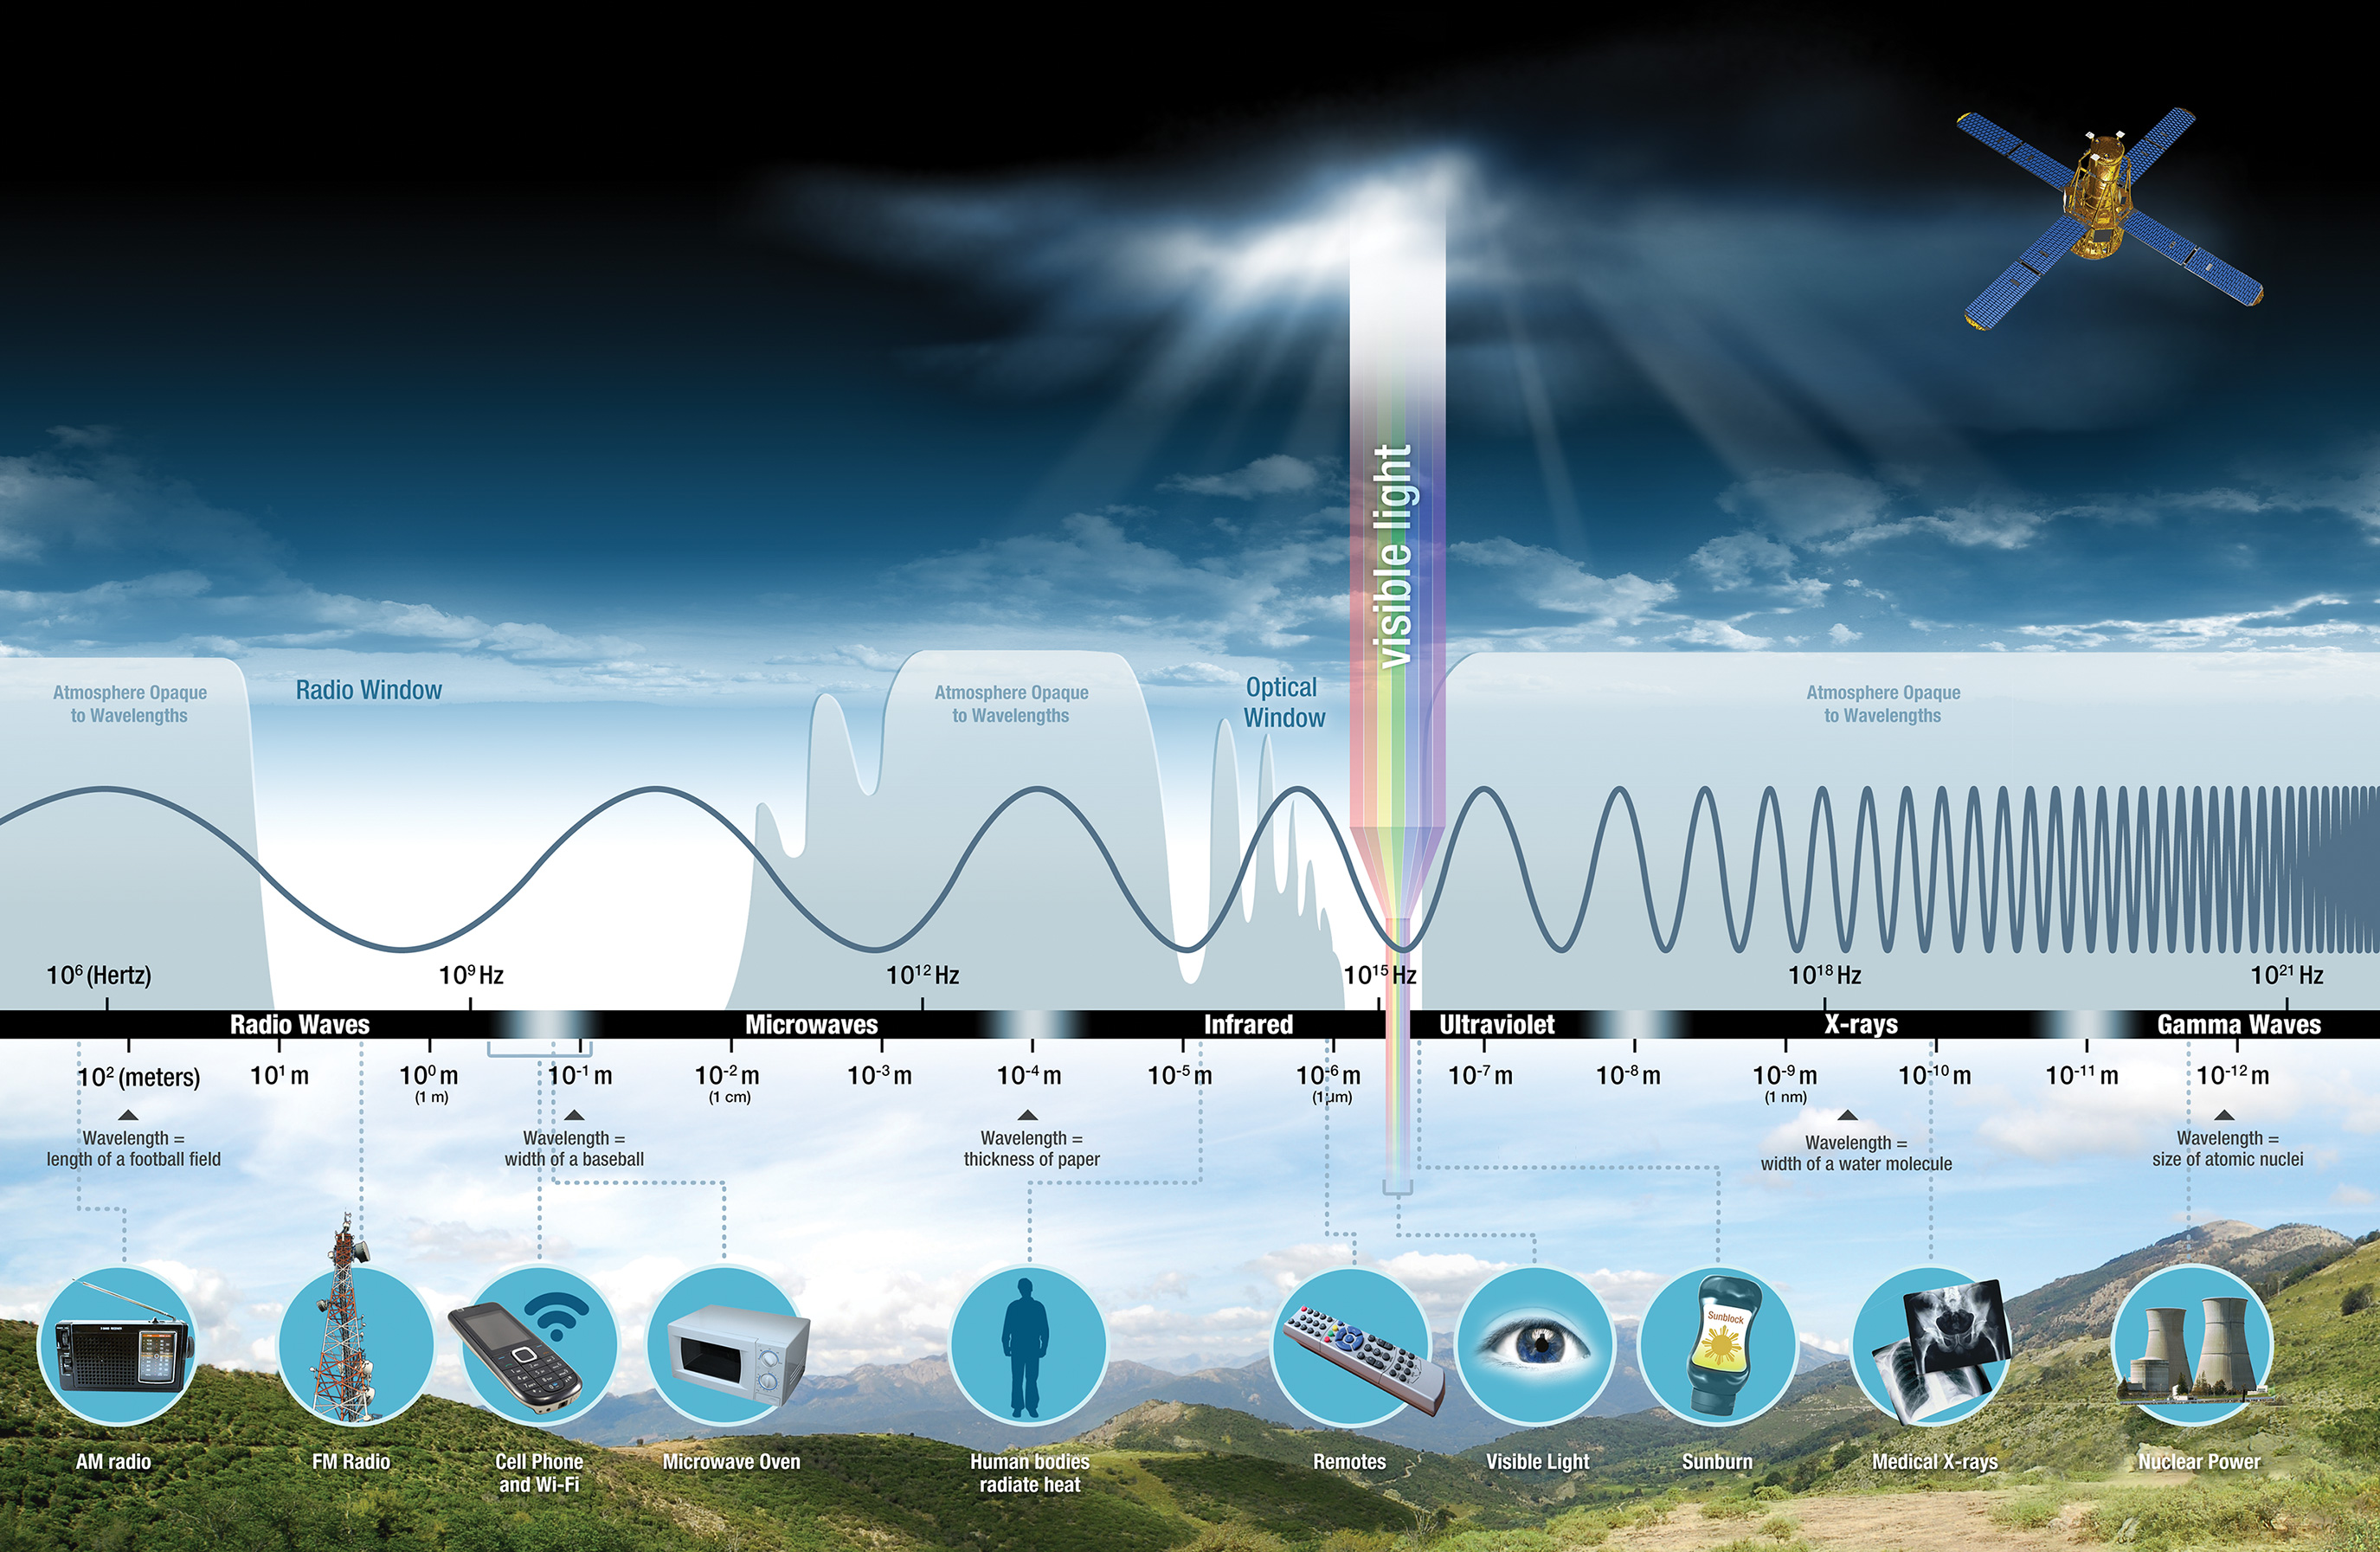
\includegraphics{./image/Diagram of the Electromagnetic Spectrum.jpeg}

}

\caption{the electromagnetic spectrum}

\end{figure}

\begin{tcolorbox}[enhanced jigsaw, title=\textcolor{quarto-callout-tip-color}{\faLightbulb}\hspace{0.5em}{Tip}, coltitle=black, opacitybacktitle=0.6, toprule=.15mm, leftrule=.75mm, opacityback=0, arc=.35mm, breakable, colbacktitle=quarto-callout-tip-color!10!white, colback=white, bottomrule=.15mm, bottomtitle=1mm, toptitle=1mm, titlerule=0mm, rightrule=.15mm, left=2mm, colframe=quarto-callout-tip-color-frame]
The magnitude of energy that an object reflects or emits across a range
of wavelengths is called its spectral response pattern/spectral
signatures. It can be used to identify objects.
\end{tcolorbox}

\textbf{Resolution}

In remote sensing we refer to three types of resolution: spatial,
spectral and temporal. Spatial Resolution refers to the size of the
smallest feature that can be detected by a satellite sensor or displayed
in a satellite image. It is usually presented as a single value
representing the length of one side of a square.
\href{https://cimss.ssec.wisc.edu/sage/remote_sensing/lesson3/concepts.html}{Remote
Sensing » Spatial Analysis}

\hypertarget{rs-data-download}{%
\subsection{RS data download}\label{rs-data-download}}

We can use:

\href{https://scihub.copernicus.eu/dhus/\#/home}{Copernicus Open Accesss
Hub} to download RS images collected by Sentinel Series Satellite.

\begin{tcolorbox}[enhanced jigsaw, title=\textcolor{quarto-callout-note-color}{\faInfo}\hspace{0.5em}{Note}, coltitle=black, opacitybacktitle=0.6, toprule=.15mm, leftrule=.75mm, opacityback=0, arc=.35mm, breakable, colbacktitle=quarto-callout-note-color!10!white, colback=white, bottomrule=.15mm, bottomtitle=1mm, toptitle=1mm, titlerule=0mm, rightrule=.15mm, left=2mm, colframe=quarto-callout-note-color-frame]
For \href{https://zhuanlan.zhihu.com/p/356726375}{Sentinel Series
Satellite Overview}

PS. Very few of the links for additional information are in Chinese, as
this makes it easier for me to understand.
\end{tcolorbox}

Note when selecting products, be careful about:

\begin{itemize}
\tightlist
\item
  Satellite transit period range (e.g.~2020/01/01 - 2020/03/07)
\item
  Data type (Sentinel1/2/3) Where Sentinel2 data can be downloaded in
  types S1C (unatmospherically corrected) and S2A (atmospherically
  corrected).
\item
  Cloud cover to extent {[}0 TO 5{]}
\end{itemize}

We can also use:

\href{https://earthexplorer.usgs.gov/.}{Landsat data} to download RS
image from Landsat Series.

\hypertarget{basic-information-of-the-image}{%
\subsection{Basic information of the
image}\label{basic-information-of-the-image}}

Copernicus Open Accesss Hub

GRANULE \textgreater{} sensor number \textgreater{} IMG\_DATA
\textgreater{} R10

Then you can see the information about the bands.Including its
resolution, central wavelength and description about which wave band it
belongs to ( Blue/Green/Ted/VNIR/\ldots)

And here is a website which provides basic information from the
characteristics of satellite to its products. For example ,this is for
\href{https://eos.com/find-satellite/landsat-5-tm/}{Landsat 5 (TM)}

\hypertarget{understanding-rs-image-through-software}{%
\subsection{Understanding RS image through
software}\label{understanding-rs-image-through-software}}

\textbf{QGIS}

\begin{tcolorbox}[enhanced jigsaw, title=\textcolor{quarto-callout-tip-color}{\faLightbulb}\hspace{0.5em}{Tip}, coltitle=black, opacitybacktitle=0.6, toprule=.15mm, leftrule=.75mm, opacityback=0, arc=.35mm, breakable, colbacktitle=quarto-callout-tip-color!10!white, colback=white, bottomrule=.15mm, bottomtitle=1mm, toptitle=1mm, titlerule=0mm, rightrule=.15mm, left=2mm, colframe=quarto-callout-tip-color-frame]
To process Sentinel data with QGIS, we can install Semi-Automatic
Classification Plugin (SCP) version 7.
\end{tcolorbox}

We can open monochrome images in different bands. We can also open the
TCI image, which is a True Colour Image of B02 (Blue), B03 (Green), and
B04 (Red) Bands.But the TCI has a range of pixel values from 0-255, it
is not visually clear. We can get a more realistic level of colour by
using BOA data.

\begin{tcolorbox}[enhanced jigsaw, title=\textcolor{quarto-callout-note-color}{\faInfo}\hspace{0.5em}{The BOA bands}, coltitle=black, opacitybacktitle=0.6, toprule=.15mm, leftrule=.75mm, opacityback=0, arc=.35mm, breakable, colbacktitle=quarto-callout-note-color!10!white, colback=white, bottomrule=.15mm, bottomtitle=1mm, toptitle=1mm, titlerule=0mm, rightrule=.15mm, left=2mm, colframe=quarto-callout-note-color-frame]
In the Sentinel 2 images available for download, you will find Level 1C
data and Level 2A data. 1C data are orthorectified and geometrically
refined atmospheric apparent reflectance products that are not
atmospherically corrected. 2A images are orthorectified
bottom-of-atmosphere (BOA) reflectance corrected images. What does this
mean? Unlike Class 1C, Class 2A images correspond to atmospherically
corrected images and provide reflectance data that are closer to the
real thing (and therefore have a more realistic colour level). It is
possible to distinguish between them visually (below), as a Class 2A
image is sharper, has higher brightness and contrast, and does not show
the whitish texture produced by atmospheric influences.
\end{tcolorbox}

In addition, using the \textbf{merge} tool to merge single-band images
can also obtain multi-band images. Then realize True Color Image by
selecting the red, green and blue bands.

\textbf{SNAP}

SNAP is an application developed by the European Space Agency for
processing Sentinel satellite data. We actually can open .zip file in
SNAP which is very convenient. And if unzip the file and open each .tiff
file separately, some important information will lose like the value of
wavelength.This
\href{https://www.youtube.com/watch?v=vtlN5MXYGaY}{video} can be help on
how to open Sentinel data in SNAP.

Following are some analysis we can do through the software:

\begin{itemize}
\tightlist
\item
  \textbf{Colour composites}
\end{itemize}

We can achieve different band combinations by selecting different remote
sensing image bands in RGB channels

\begin{tcolorbox}[enhanced jigsaw, title=\textcolor{quarto-callout-tip-color}{\faLightbulb}\hspace{0.5em}{Tip}, coltitle=black, opacitybacktitle=0.6, toprule=.15mm, leftrule=.75mm, opacityback=0, arc=.35mm, breakable, colbacktitle=quarto-callout-tip-color!10!white, colback=white, bottomrule=.15mm, bottomtitle=1mm, toptitle=1mm, titlerule=0mm, rightrule=.15mm, left=2mm, colframe=quarto-callout-tip-color-frame]
Be careful that different RS data may have different meanings for the
band with the same No.~
\end{tcolorbox}

For Sentinel 2 data:

\begin{longtable}[]{@{}
  >{\raggedright\arraybackslash}p{(\columnwidth - 4\tabcolsep) * \real{0.3571}}
  >{\raggedright\arraybackslash}p{(\columnwidth - 4\tabcolsep) * \real{0.3333}}
  >{\raggedright\arraybackslash}p{(\columnwidth - 4\tabcolsep) * \real{0.3095}}@{}}
\caption{Sentinel 2 Bands and Combinations}\tabularnewline
\toprule()
\begin{minipage}[b]{\linewidth}\raggedright
Types
\end{minipage} & \begin{minipage}[b]{\linewidth}\raggedright
RGB channels
\end{minipage} & \begin{minipage}[b]{\linewidth}\raggedright
description
\end{minipage} \\
\midrule()
\endfirsthead
\toprule()
\begin{minipage}[b]{\linewidth}\raggedright
Types
\end{minipage} & \begin{minipage}[b]{\linewidth}\raggedright
RGB channels
\end{minipage} & \begin{minipage}[b]{\linewidth}\raggedright
description
\end{minipage} \\
\midrule()
\endhead
Natural Color & B4, B3, B2 & display imagery the same way our eyes see
the world \\
Color Infrared & B8, B4, B3 & emphasize healthy and unhealthy
vegetation. denser vegetation is red,but urban areas are white \\
Agriculture & B11,B8,B2 & used to monitor the health of
crops,highlighting dense vegetation that appears as dark green \\
Geology & B12, B11, B2 & for finding geological features. This includes
faults, lithology, and geological formations \\
\bottomrule()
\end{longtable}

For Landsat 5 TM data:

\begin{longtable}[]{@{}
  >{\raggedright\arraybackslash}p{(\columnwidth - 4\tabcolsep) * \real{0.3571}}
  >{\raggedright\arraybackslash}p{(\columnwidth - 4\tabcolsep) * \real{0.3333}}
  >{\raggedright\arraybackslash}p{(\columnwidth - 4\tabcolsep) * \real{0.3095}}@{}}
\caption{Landsat 5 TM Bands and Combinations}\tabularnewline
\toprule()
\begin{minipage}[b]{\linewidth}\raggedright
Types
\end{minipage} & \begin{minipage}[b]{\linewidth}\raggedright
RGB channels
\end{minipage} & \begin{minipage}[b]{\linewidth}\raggedright
description
\end{minipage} \\
\midrule()
\endfirsthead
\toprule()
\begin{minipage}[b]{\linewidth}\raggedright
Types
\end{minipage} & \begin{minipage}[b]{\linewidth}\raggedright
RGB channels
\end{minipage} & \begin{minipage}[b]{\linewidth}\raggedright
description
\end{minipage} \\
\midrule()
\endhead
Natural Color & B3, B2, B1 & display imagery the same way our eyes see
the world \\
Standard false color & B4, B3, B2 & emphasize healthy and unhealthy
vegetation. denser vegetation is red,but urban areas are white \\
simulated true color & B7,B4,B3 & Identify residential land and water
bodies \\
\ldots{} & \ldots{} & \ldots{} \\
\bottomrule()
\end{longtable}

\begin{figure}

{\centering \includegraphics{./image/1.png}

}

\caption{Color Infrared}

\end{figure}

\begin{tcolorbox}[enhanced jigsaw, title=\textcolor{quarto-callout-tip-color}{\faLightbulb}\hspace{0.5em}{Tip}, coltitle=black, opacitybacktitle=0.6, toprule=.15mm, leftrule=.75mm, opacityback=0, arc=.35mm, breakable, colbacktitle=quarto-callout-tip-color!10!white, colback=white, bottomrule=.15mm, bottomtitle=1mm, toptitle=1mm, titlerule=0mm, rightrule=.15mm, left=2mm, colframe=quarto-callout-tip-color-frame]
In addition to band combination, we can also use some band calculations
to obtain images that can highlight targets.For example, Vegetation
Index (B8-B4)/(B8+B4), Moisture Index (B8A-B11)/(B8A+B11)
\end{tcolorbox}

\begin{itemize}
\tightlist
\item
  \textbf{Image statistics}
\end{itemize}

\textbf{Histogram}

A graph that describes the relationship between each gray level in an
image and its frequency of occurrence. Histograms for each band of the
image can be viewed in SNAP. If we change the mapping range of image
pixels in 0-255, the image will be changed visually. We generally omit
1\% at the lower end and 4\% at the upper end for mapping. In addition,
image contrast can be improved by adjusting the histogram morphology.

\begin{tcolorbox}[enhanced jigsaw, title=\textcolor{quarto-callout-note-color}{\faInfo}\hspace{0.5em}{Note}, coltitle=black, opacitybacktitle=0.6, toprule=.15mm, leftrule=.75mm, opacityback=0, arc=.35mm, breakable, colbacktitle=quarto-callout-note-color!10!white, colback=white, bottomrule=.15mm, bottomtitle=1mm, toptitle=1mm, titlerule=0mm, rightrule=.15mm, left=2mm, colframe=quarto-callout-note-color-frame]
Mean: reflects the overall brightness of the image

Variance: refers to the variance of the brightness value of each band,
reflecting the volume of the information
\end{tcolorbox}

\textbf{Scatterplot}

The scatterplot is used to analyze the spatial distribution relationship
between two bands. For example, draw a scatter diagram of red
(vegetation absorbs) and Near-infrared (NIR, that vegetation strongly
reflects). Since higher NIR values and lower red values indicate dense
vegetation, while lower values of both are usually bare soil. Therefore,
the image can roughly analyze the distribution characteristics of
different ground objects.

\begin{figure}

{\centering 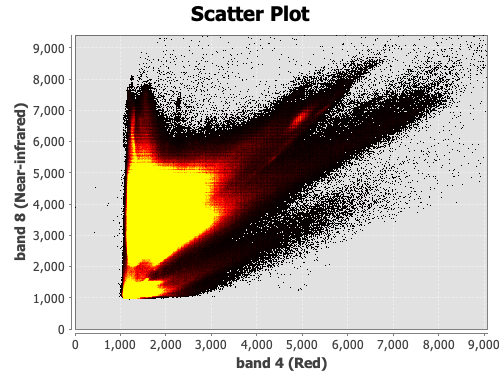
\includegraphics{./image/scatterplot.png}

}

\caption{Scatter Plot}

\end{figure}

\begin{itemize}
\tightlist
\item
  \textbf{Masking and resampling}
\end{itemize}

Remote sensing images can be cropped using vector data (Raster
\textgreater{} Masks \textgreater{} Land/Sea mask) to leave areas of
interest. Note that SNAP can only read ESRI shapefiles. In addition,
before cropping, we need to unify the resolution of the band, you can
use the resampling tool (Raster \textgreater{} Geometric \textgreater{}
Resampling)

\begin{itemize}
\tightlist
\item
  \textbf{Comparison of spectral signatures}
\end{itemize}

We can extract the spectral signatures of different land cover classes
using the Semi-automatic Classification plugin in QGIS 3.16. Here is a
\href{https://www.youtube.com/watch?v=Myd-rgxRTfI}{tutorial video}

\begin{figure}

{\centering 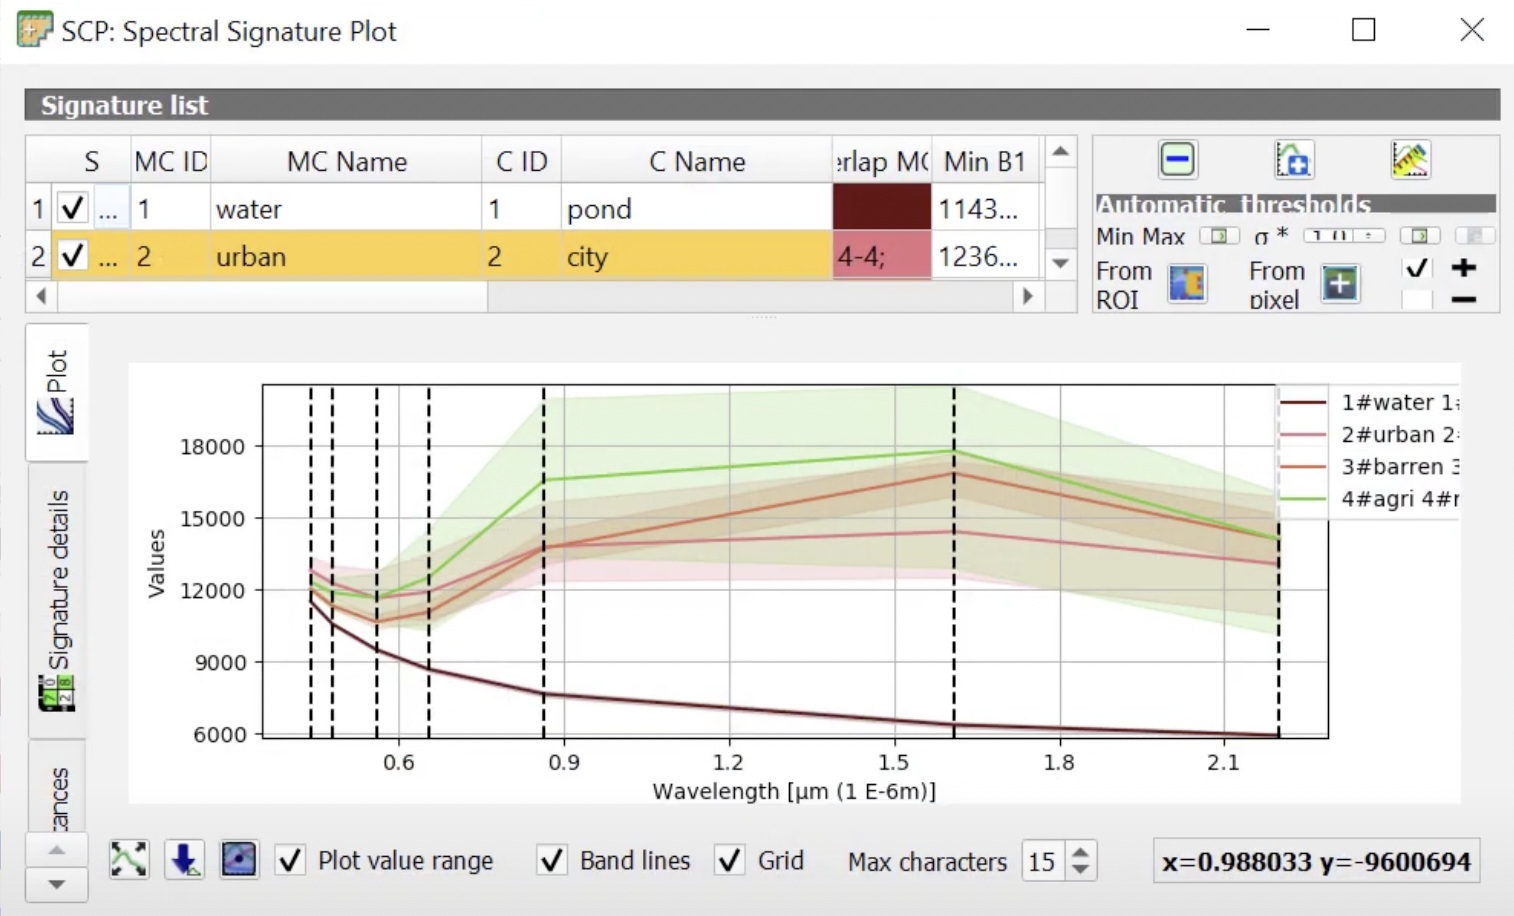
\includegraphics{./image/spectral signature.png}

}

\caption{Spectral Signatures in QGIS}

\end{figure}

Also, it is easy to do it in SNAP. Basically you just need to use
Optical-\textgreater Spectrum View, and make sure that your image has
band information. Besides, you can use Pin tool to make sample, and
compare the curve of different objects. Here is another tutorial video
about \href{https://www.youtube.com/watch?v=5znAQH6vrLs}{Pins and
Spectrum Tool in SNAP}

\begin{figure}

{\centering 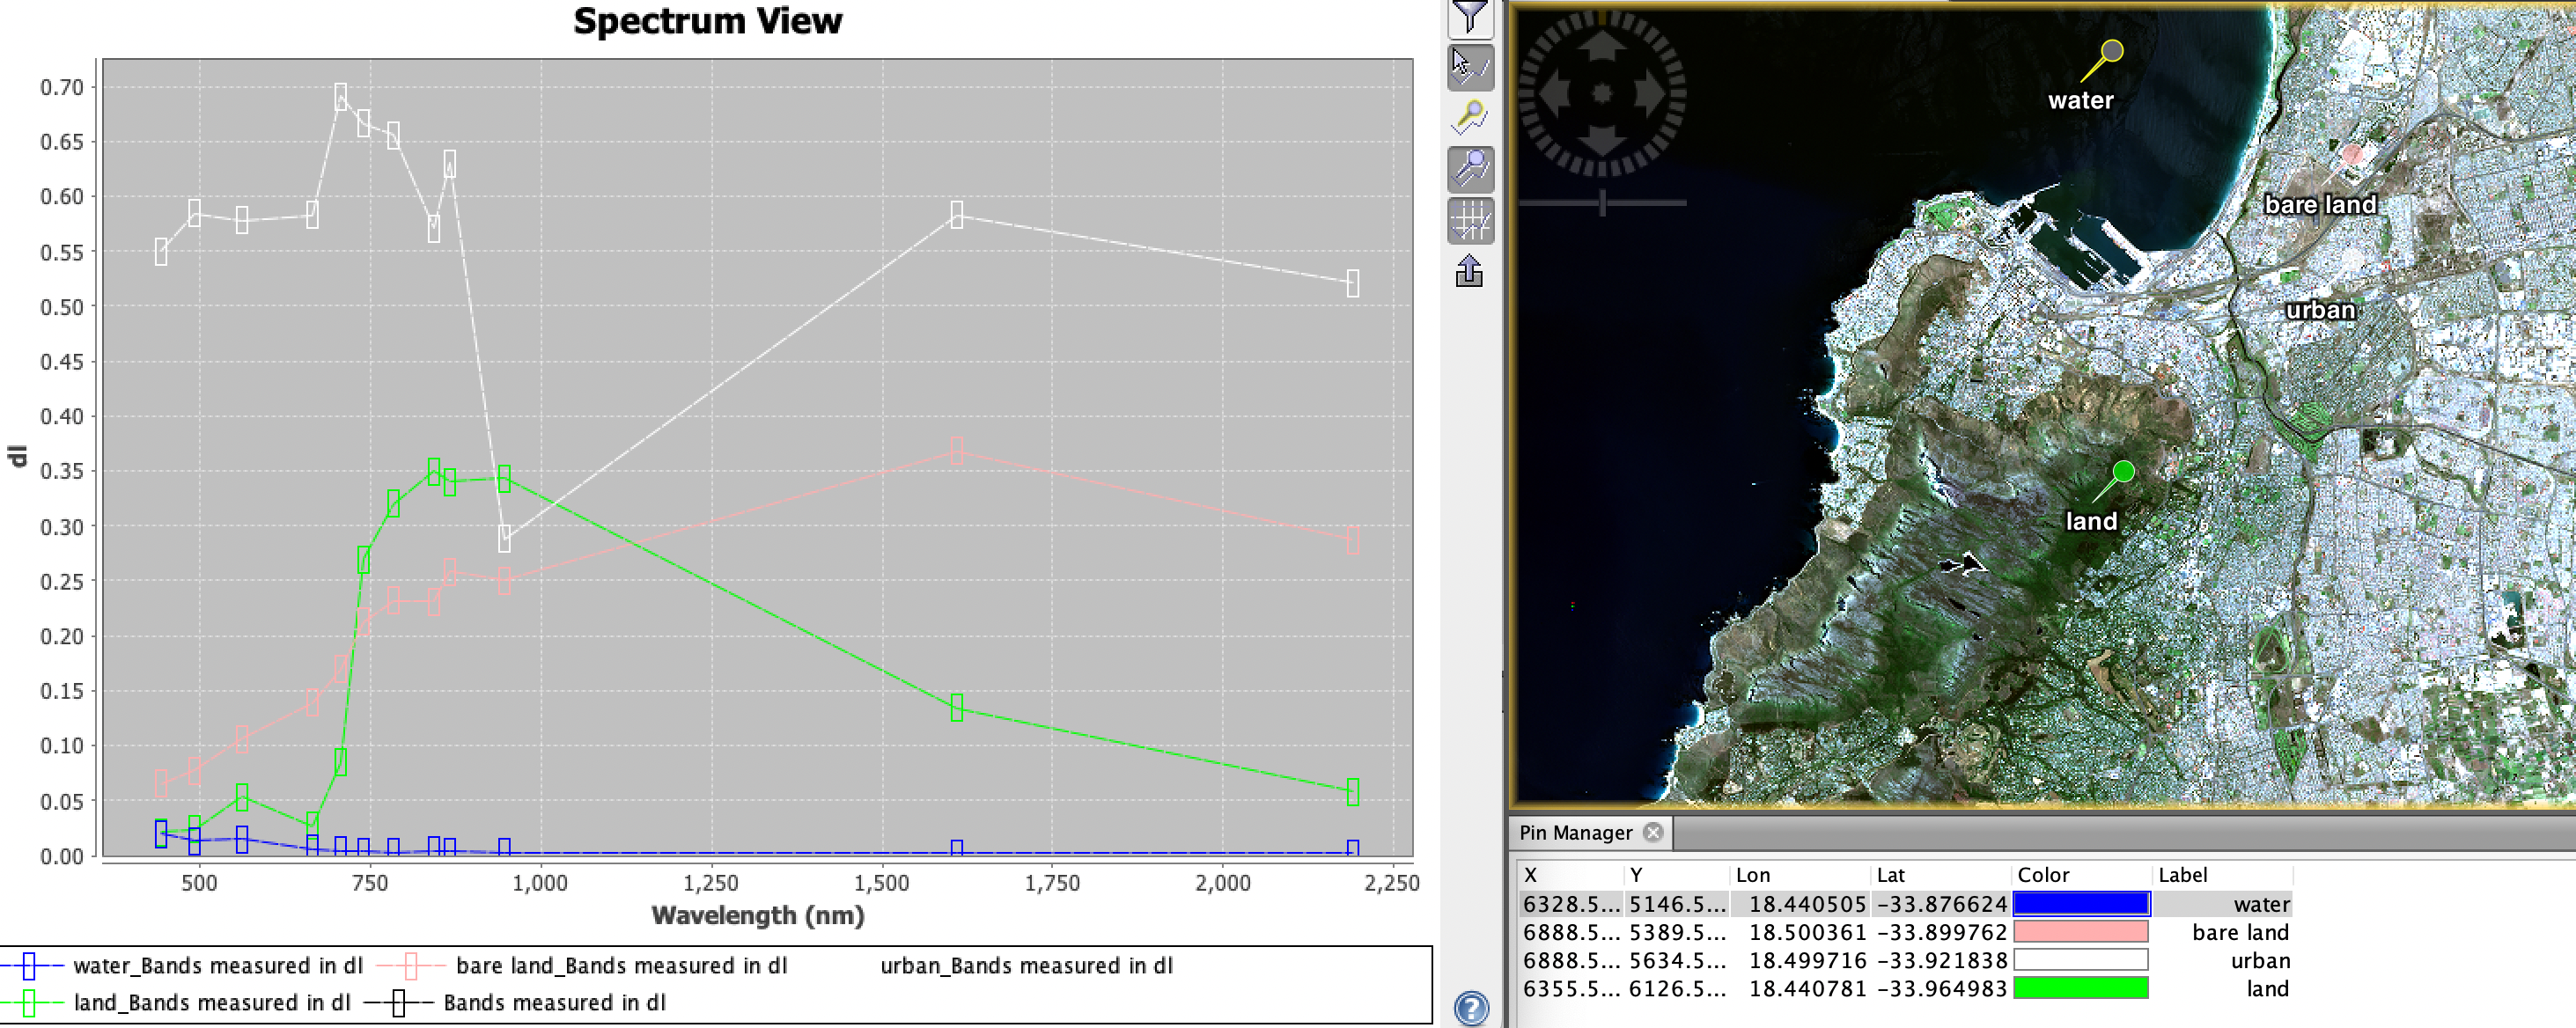
\includegraphics{./image/SNAP1.png}

}

\caption{Spectrum View in SNAP}

\end{figure}

\hypertarget{application}{%
\section{Application}\label{application}}

The main application of Remote Sensing Image is about recognizing
geographical entities, which is well used in agriculture, forestry,
geology, marine, meteorology, hydrology, military, environmental
protection and other fields.Here, I will give same simple example of how
we use remote sensing image in \textbf{agriculture} scenarios.

\begin{figure}

{\centering \includegraphics{./image/application1.webp}

}

\caption{Using RS to predict corn harvest time, Source:
\href{https://doi.org/10.3390/rs13101878}{Janoušek et al.~2021}}

\end{figure}

\emph{Crop remote sensing production estimation is based on the
collection of different spectral signatures of various crops in
different growth stages according to biological principles, through the
surface information recorded by the sensor on the platform, to identify
crop types, monitor crop growth, and predict crop yield before crop
harvest a range of methods. This technology can dynamically monitor the
growth process of crops, measure the planting area, estimate the output
per unit area and estimate the total output.}

Traditionally, optical and infrared sensors will be used to
\textbf{detect the irrigated areas}, for example,
\href{https://doi.org/10.1016/j.rse.2004.12.018}{Thenkabail et
al.~(2005)} developed a comprehensive algorithm based on timeseries of
MODIS spectral bands (2, 3, 5, 6, and 7) data to detect irrigation and
rainfed classes along with crop onset, peak, and senescence (aging of
the plant).

And for \textbf{crop yield assessment}, using remote sensing of plant
photosynthetic activity is a good way as photosynthetic activity
influences biomass production. Both passive and active microwave remote
sensing can help us to do it. There are some indicators or models like
the Vegetation Optical Depth (VOD)
\href{https://doi.org/10.1016/j.rse.2015.10.021}{(Guan et al.~2016)}.
Besides, regression relationship with indices such as NDVI, RVI, and VCI
are used to estimate crop yield.

\begin{figure}

{\centering \includegraphics{./image/application1.2.webp}

}

\caption{Source: \href{https://doi.org/10.3390/rs12233945}{Tolomio et
al.~2020}}

\end{figure}

In addition, remote sensing technology can also be useful when
\textbf{detecting agricultural pests and diseases}. Indices such as
Disease Water Stress Index (DWSI) , Disease Index (DI) and Yellow Rust
Index (YRI) for detecting wheat yellow rust, Aphid Index (AI), and
Leafhopper Index (LHI) , among others are proposed for pest and disease
detection
\href{https://doi.org/10.1016/j.jhydrol.2020.124905}{(Karthikeyan et
al.~2020)}.

\hypertarget{reflection}{%
\section{Reflection}\label{reflection}}

\begin{itemize}
\item
  For remote sensing image data, the products generated by different
  sensors are very different, such as the information of bands and the
  structure of downloaded files. This requires us to have a good
  understanding of these video products before processing the data,
  otherwise you don't even know how to open them in the software.
\item
  As for software, these software are not very friendly to novices, such
  as densely packed menu bars and tools that don't know where they are.
  Fortunately, YouTube has many tutorials to help you operate.
\item
  The subject of remote sensing involves some physical knowledge, such
  as spectrum and radiation, which is sometimes a bit difficult to
  understand. The remote sensing of the visible light part can be
  interpreted through eyes which is helpful to understand. Others, such
  as microwave remote sensing, are even more difficult to understand.
\item
  However, when I was studying agricultural remote sensing, I felt the
  power of this technology. When the study area is large, remote sensing
  is a good choice to monitor dynamic changes. Moreover, it can digitize
  the characteristics of geographic entities, such as the reflectivity
  of the electromagnetic spectrum with different wavelengths. This
  digitization provides opportunities for further data analysis (and the
  scale of the data is easily consistent, this is great). Therefore, a
  large number of ML and AI technologies are applied to remote sensing
  image processing. This brings greater promise to the application of
  remote sensing.
\end{itemize}

\hypertarget{reference}{%
\section{Reference}\label{reference}}

~~~~~~~~Janoušek, Jiří, et al.~``Using UAV-based photogrammetry to
obtain correlation between the vegetation indices and chemical analysis
of agricultural crops.'' \emph{Remote Sensing} 13.10 (2021): 1878.\\
\hspace*{0.333em}\hspace*{0.333em}\hspace*{0.333em}\hspace*{0.333em}\hspace*{0.333em}\hspace*{0.333em}\hspace*{0.333em}\hspace*{0.333em}Grant,
J. P., et al.~``Comparison of SMOS and AMSR-E vegetation optical depth
to four MODIS-based vegetation indices.'' \emph{Remote Sensing of
Environment} 172 (2016): 87-100.\\
\hspace*{0.333em}\hspace*{0.333em}\hspace*{0.333em}\hspace*{0.333em}\hspace*{0.333em}\hspace*{0.333em}\hspace*{0.333em}\hspace*{0.333em}Thenkabail,
Prasad S., Mitchell Schull, and Hugh Turral. ``Ganges and Indus river
basin land use/land cover (LULC) and irrigated area mapping using
continuous streams of MODIS data.'' \emph{Remote Sensing of Environment}
95.3 (2005): 317-341.\\
\hspace*{0.333em}\hspace*{0.333em}\hspace*{0.333em}\hspace*{0.333em}\hspace*{0.333em}\hspace*{0.333em}\hspace*{0.333em}\hspace*{0.333em}Karthikeyan,
L., Ila Chawla, and Ashok K. Mishra. ``A review of remote sensing
applications in agriculture for food security: Crop growth and yield,
irrigation, and crop losses.'' \emph{Journal of Hydrology} 586 (2020):
124905.\\
\hspace*{0.333em}\hspace*{0.333em}\hspace*{0.333em}\hspace*{0.333em}\hspace*{0.333em}\hspace*{0.333em}\hspace*{0.333em}\hspace*{0.333em}Huang,
Jianxi, et al.~``Assimilation of remote sensing into crop growth models:
Current status and perspectives.'' \emph{Agricultural and Forest
Meteorology} 276 (2019): 107609.\\
\hspace*{0.333em}\hspace*{0.333em}\hspace*{0.333em}\hspace*{0.333em}\hspace*{0.333em}\hspace*{0.333em}\hspace*{0.333em}\hspace*{0.333em}Tolomio,
Massimo, and Raffaele Casa. ``Dynamic crop models and remote sensing
irrigation decision support systems: A review of water stress concepts
for improved estimation of water requirements.'' \emph{Remote Sensing}
12.23 (2020): 3945.

And some other website may be useful:
\href{https://gisgeography.com/}{Learn GIS and Geography}

\bookmarksetup{startatroot}

\hypertarget{week2}{%
\chapter{WEEK2}\label{week2}}

This week is about Xaringan and Quarto 1 2 3 4

\bookmarksetup{startatroot}

\hypertarget{references}{%
\chapter*{References}\label{references}}
\addcontentsline{toc}{chapter}{References}

\hypertarget{refs}{}
\begin{CSLReferences}{0}{0}
\end{CSLReferences}



\end{document}
